\subsection{Streaming}\label{sec:design-stream}

The proposed design distinguishes between its \textit{core} overlay mesh and the \glsfirst{dag} of streaming connections as shown in \vref{fig:stream-graph}. The overlay mesh keeps track of node presence, their respective connection quality and delivers messages. The streaming \gls{dag} establishes additional unidirectional connections to distribute audio and video tracks across nodes.

\begin{figure}
\centering
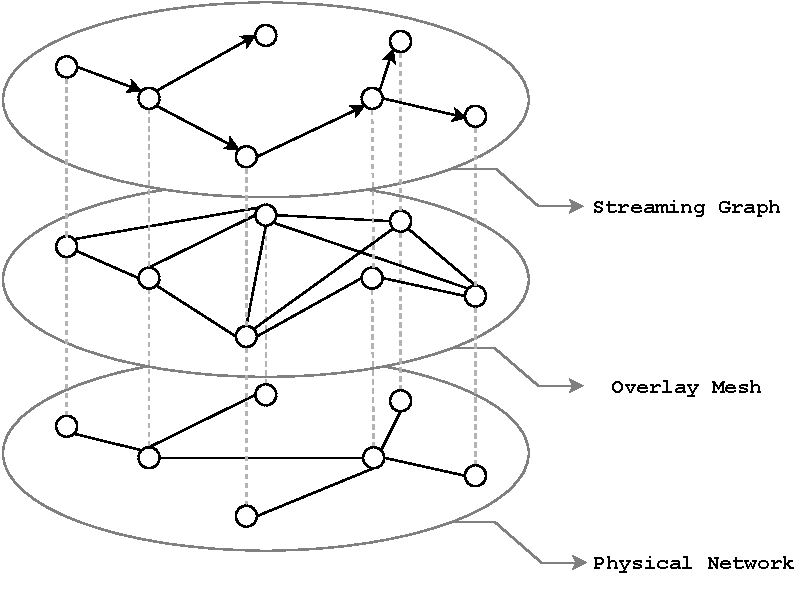
\includegraphics[width=.75\textwidth]{graphics/design/stream-graph.pdf}
\caption{Layering of the physical, mesh and streaming network}
\label{fig:stream-graph}
\end{figure}

Allowing multiple nodes to propagate their streams, requires the system to distinguish between multiple content sources. To that end, the design introduces the concepts of channels and providers. Every node that starts a media stream creates a new channel and every node that has active access to a channel becomes a provider. All nodes keep track of channels and providers in their periphery to see what content is available and from whom.

\subsubsection{Channels}\label{sec:design-stream-channel}
A channel is assigned a \gls{uuid} on creation and can carry further application–specific data. Peers announce the existence of channels in periodic updates \ref{item:peer-publish-channel-announcement} to their direct connections. This way channels announcements are gossiped \cref{gossiping} through the network and will eventually \textit{infect} all nodes. The application or its user can then decide which channel to watch and the system will try to acquire a stream connection for it.

\subsubsection{Provider}\label{sec:design-stream-provider}
Nodes need to keep track of who is in possession of an active stream source and who has upload capacity to provide them the stream. Therefore, nodes advertise upload capacity in their \glspl{channel-announcement}. Because upload capacity can vary between nodes, they need to estimate, how many downstream nodes they can supply, themselves. Additionally, nodes should propagate their distance from the original stream source. This will be an essential metric for \gls{dag} creation.

Analogous to the overlay mesh, the streaming \gls{dag} has to be constructed, maintained and downsized by the nodes it consists of. Again, there is no central point of knowledge, that could construct an optimal graph. Nodes have to act on their own and the decision which paths to take, is distributed across the overlay.

\subsubsection{Construction}\label{sec:design-stream-construction}
The streaming network is constructed on–demand using the underlying mesh network. Two strategies are employed to achieve a swift and stable saturation.
\citet*[\S3]{push-to-pull} introduce a protocol with a push and pull strategy to give all nodes access to blocks of live streaming media. In a first round, the stream source, pushes blocks to a set of nodes that themselves then pushes the blocks to other nodes. This recursive procedure is performed a predefined number of times and nodes are selected based on a \gls{dht}–style ID prefix \ref{dht}. This push strategy wants to provide a base saturation that is ahead of the actual demand. Thus, when the demand rises, the blocks are available on more devices than just the producer. \citet{push-to-pull} then use a second round to let all other nodes pull in the blocks from their vicinity. This technique can not be directly applied to this design because of the requirement for browser compatibility (see \vref{sec:requirements}). Firstly, connection establishment is much more costly and nodes cannot instantly connect to arbitrary nodes with just their address. Nodes need their mesh network to exchange negotiations, so \textit{random access} becomes fragile and time consuming.
Secondly, splitting up live streams into blocks is only possible with \glsfirst{mse} and the \textit{Media Recorder} \gls{api}, which is lacking wide browser support \cref{par:browser-media-mse}. Even if recording blocks of media would be widely supported, it still adds significant latency and restoring a smooth playback experience in browser is non–trivial. Blocks have to be prioritised, kept in order, and audio and video has to be synchronised with in–codec time codes.
In contrast, the browser's \gls{webrtc} \gls{api} provides all this, as a transparent service \ref{sec:webrtc}.

So, the push and pull phases must be adapted to continuous \gls{webrtc} stream connections and node selection has to be restricted to nodes that are reachable with just a few or zero hops.

\paragraph{Push Strategy}\label{par:design-stream-construction-push}
In the push phase, each node – starting with the stream creator – selects \outStreamConnections of its adjacent nodes to push the stream to. Candidates are selected based on connection quality estimates based on responsiveness and latency. The selected nodes receive a \gls{connection-negotiation} offer with the channel \gls{uuid} and an \gls{sdp} payload containing \gls{ice} candidates and media descriptors. The node then decides whether it has capacity to forward the stream or if it has reached its upper bound for inbound stream connections \inStreamConnections. It can also decline the offer, if it already has an active provider for this channel. This way, the streaming graph is kept loop–free i.e. acyclical. The push phase ends when all branches have run into such a dead end or if the pushed stream has passed a maximum number of hops. The risk, that this phase might terminate unintentionally early because of rejections, will be tolerated. It bears the benefit, that peers do not need to await and handle rejections and can initiate the second phase instantly.

\paragraph{Pull Strategy}\label{par:design-stream-construction-pull}
In the second phase, a pull strategy is applied to allow nodes to acquire an uplink to the stream, based on demand. They receive channel announcements and let the higher level application or a user interaction decide which channel is of interest. They send connection requests to nodes that advertised upload capacity and are provided with the stream. Subsequently, they also start advertising capacity and allow their neighbours to retrieve the stream from them. The pull strategy also comes into play, should any of the connections fail. Since nodes already know who can provide an alternative streaming path, they can recover by switching the uplink. Depending on a node's download capacity and overall channel count, nodes could even keep a \textit{hot stand–bye} connection to an alternate stream provider and switch over even quicker.

\subsubsection{Graph properties}\label{sec:design-stream-graph}

The edges of the streaming graphs do not need to align with the edges of the mesh. Both change over time and adapt to nodes joining or leaving. The streaming graphs are constructed per channel, so multiple streaming graphs can coexist on the same mesh. Whereas the edges of the mesh are bidirectional, the streaming graph has unidirectional, directed edges.
